\section{Introduction}
\label{sec:introduction}
Lightyear designs and develops solar electric vehicles, these are highly efficient battery powered vehicles that can charge their batteries using an integrated solar panel. The first vehicle designed by Lightyear is the \textit{Lightyear 0}, shown in Figure~\ref{fig:zero}. Some of the factors that play a role in a vehicle's efficiency are: aerodynamic drag, friction losses from tires, cabin heating and cooling, drivetrain losses and static energy consumption by the electric components. Lightyear seeks to design a vehicle that minimizes these losses, as a reduction in energy consumption creates a positive feedback loop. Resulting in a vehicle with a very low energy consumption that can generate a significant amount of range from its integrated solar panels.

\begin{figure}[htb]
    \centering
    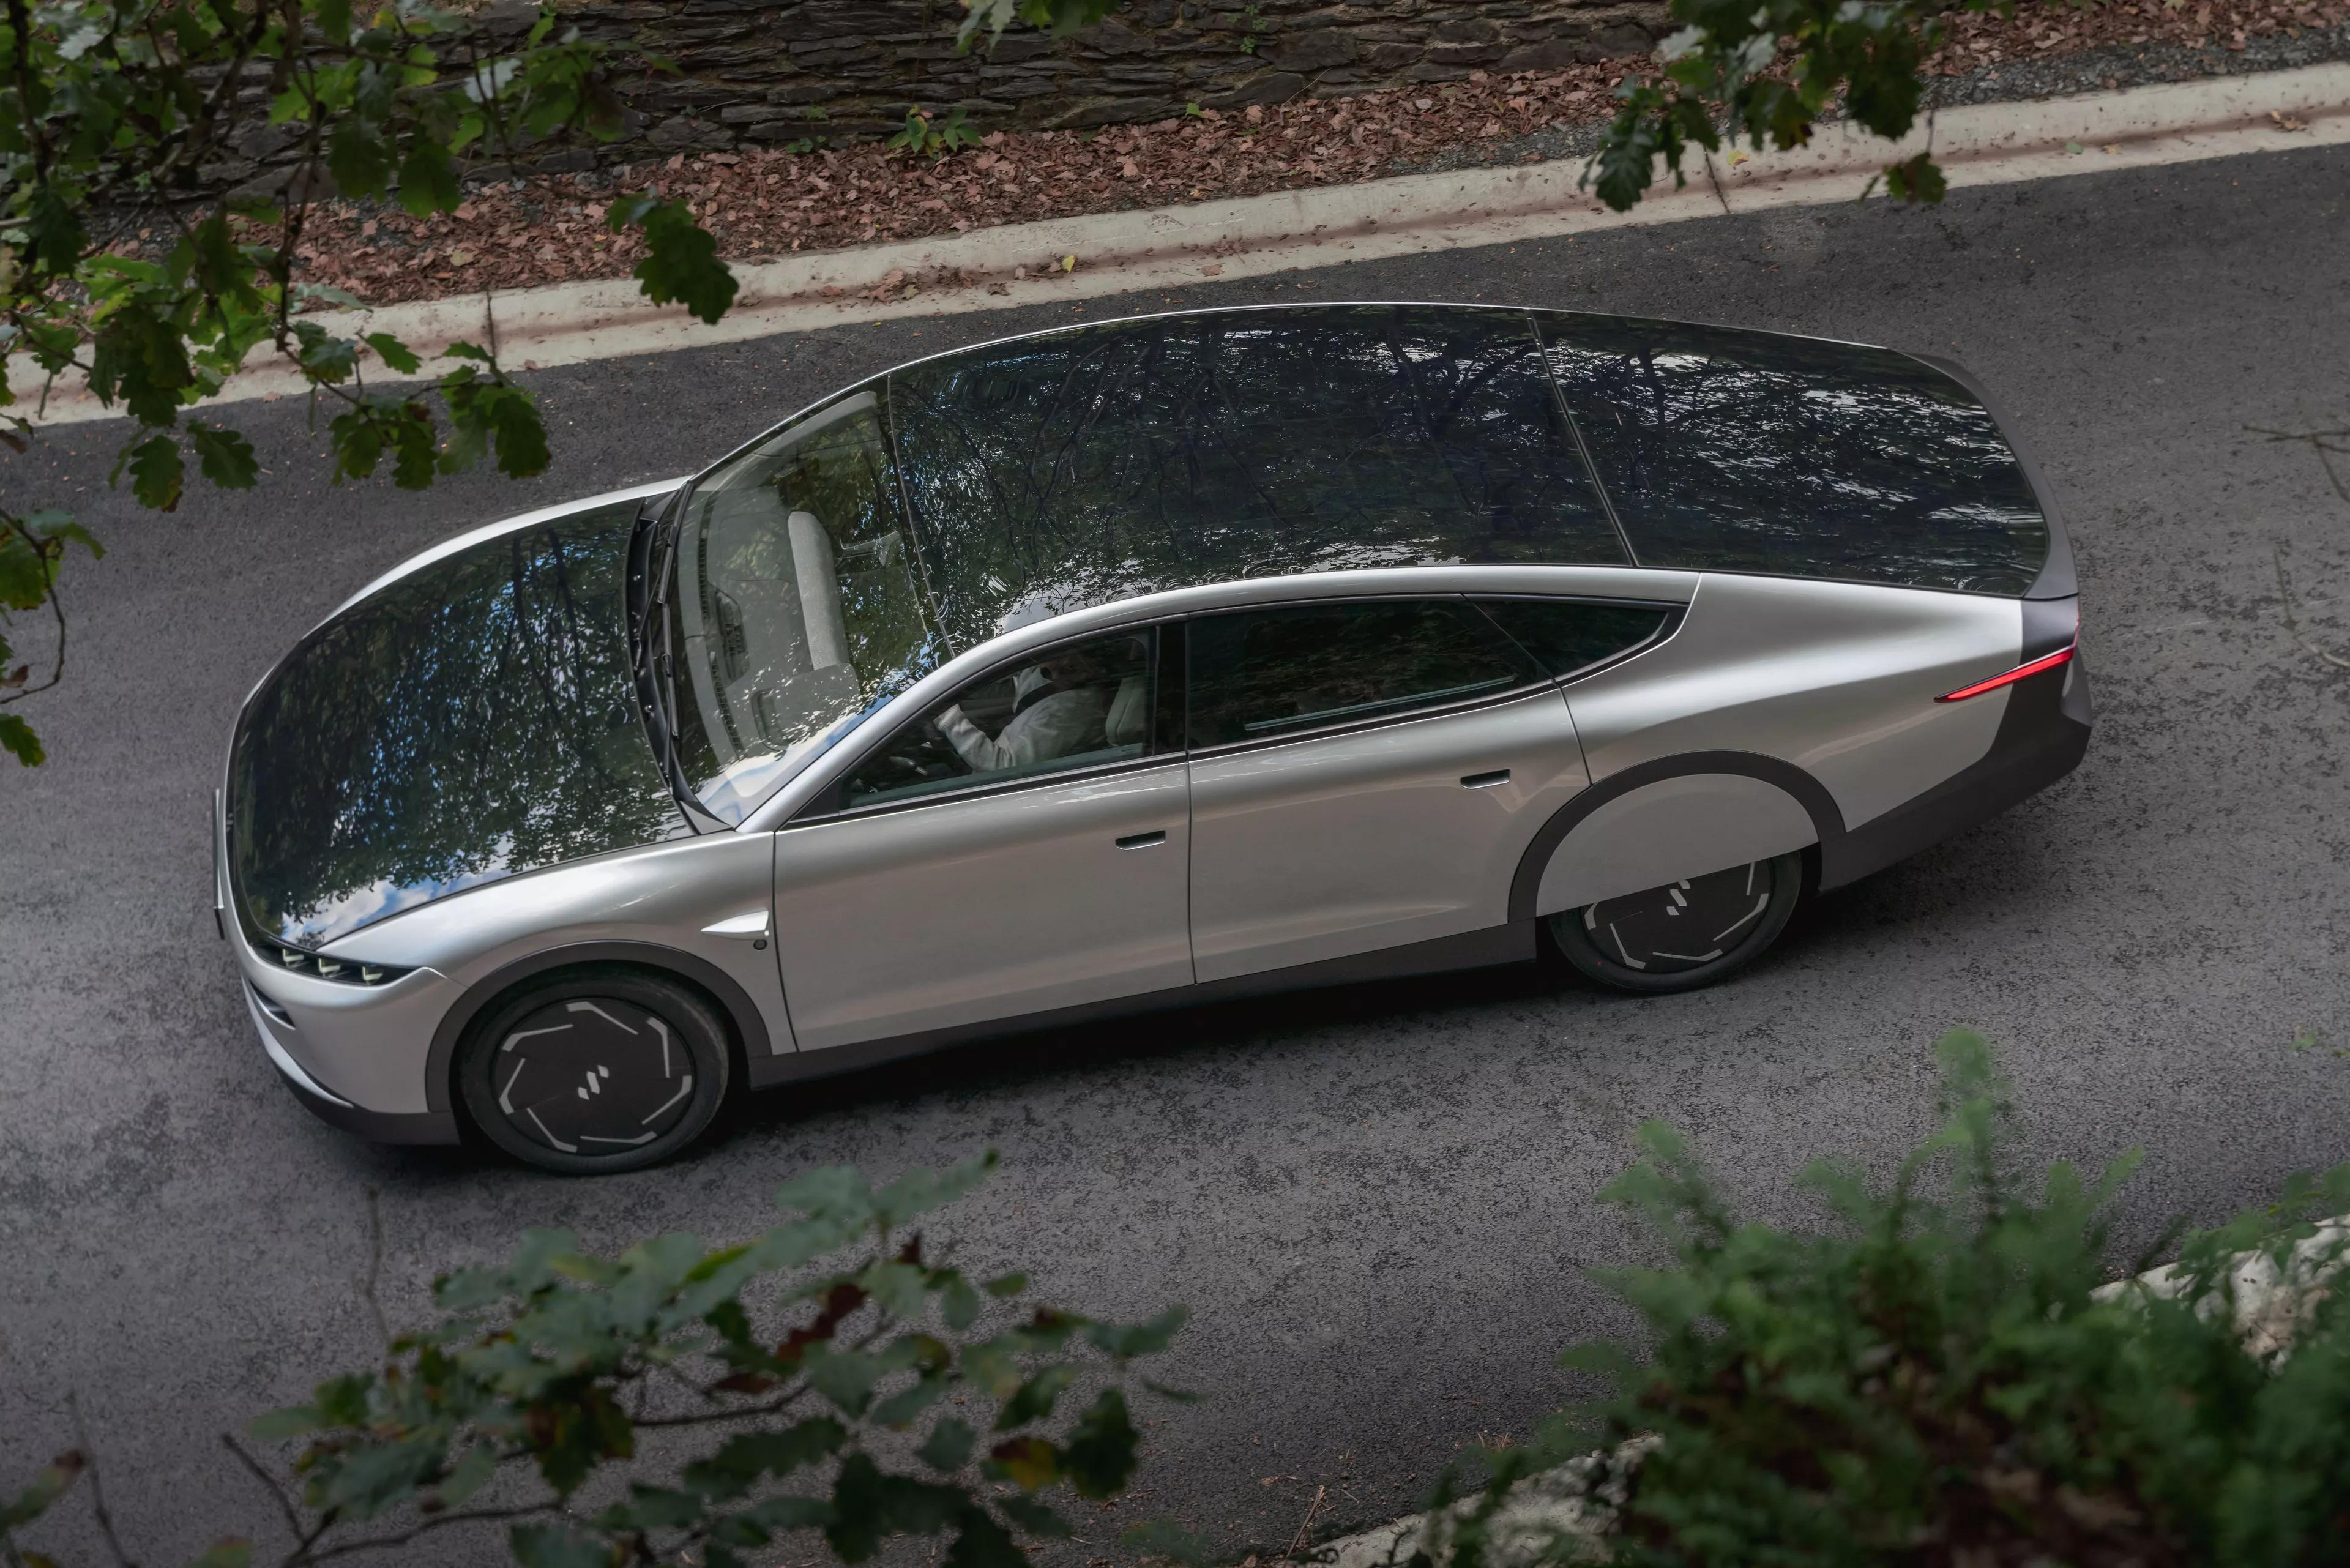
\includegraphics[width=0.9\textwidth]{images/Lightyear_zero.jpg}
    \caption{The Lightyear 0}
    \label{fig:zero}
\end{figure}

The automotive industry has recognized a need to change the vehicle architectures to leverage the Time Sensitive Networking (TSN) technology. Time Sensitive Networking is a comprehensive set of standards which can be combined and configured in various ways. The industry proposes a two-step transitioning process, starting with the introduction of a TSN backbone used by the most important nodes in the network to communicate with each other. In this stage the number of changes to the architecture and applications are kept to a minimum, focussing on the implementation of TSN. A structured approach for determining the effects of network configuration on the applications will increase the chances of success. In this report we research how simulation using the \omnet framework can be used to evaluate the effects of various network configurations on the vehicle's embedded software. Our goal is to create a model generic enough to make simulation of an entire vehicle feasible while being detailed enough to adequately answer performance questions at the system level. Available benchmarks of in-vehicle networks are sparse and do not accurately represent the Lightyear 0. We develop a method to extract a model from source code, representing the network traffic and embedded software of the Lightyear 0. The resulting model describes the inner workings of the main nodes in the network, the mapping of functionality to nodes and details the messages transmitted in the network. We show that Lightyear's application software mostly communicates in terms of \textit{data dictionaries}, representing a system state sample, and that the applications are agnostic of the network implementation. Making the architecture suitable for a transformation to a TSN based network. Finally, the model is simulated using the \omnet framework and some experiments are performed, demonstrating that simulation of an entire vehicle is both feasible and capable of answering performance questions. For example, we show that the effects of network configuration on the synchronization of data in the network can be evaluated with our model. The \omnet model and the benchmark detailing the vehicle's embedded system are publicly available on Github\footnote{\url{https://github.com/StephanOostveen/graduation}}

Section~\ref{sec:domain} gives some background information on the automotive industry: communication networks used, current and future architectures. Section~\ref{sec:problem_statement} presents Lightyear's challenges, the overarching problem that needs to be solved, and possible directions of research. Section~\ref{sec:sota} analyses the available automotive benchmarks, analysis methods of CAN and TSN and simulation methods in literature. Section~\ref{sec:research_description} defines the scope of the project and the expected contributions to the problem statement. In section~\ref{subsec:network} we describe the in-vehicle network and execution model of the nodes in the network. The presented information is reverse-engineered from source code, documentation and meetings with developers. The implementation of the model in the \omnet framework is described in section~\ref{subsec:moddeling}. In section~\ref{subsec:model_gen} we describe the automatic solution for retrieving the application characteristics from the source code and why this works for Lightyear and other users of the OpenECU real time operating system. Section~\ref{sec:results} presents the retrieved benchmark and demonstrates the possible analyses that can be performed with the \omnet model. Section~\ref{sec:discussion} discusses the results, evaluates the approach and explains how the model can be changed to accommodate TSN.